\chapter{Web Programming}

\section{Overview}

Due to the ubiquity of the world wide web (WWW or ``web'' for short),
many applications offer web-based interfaces in order to support
convenient access to them. This chapter describes how one can
implement web-based interfaces in Curry. We will see that
the functional and logic programming features of Curry
are quite useful in providing a high-level programming interface
for such applications so that Curry can also be used as
a language for ``web scripting,'' i.e., for writing web interfaces
in a concise manner.

This chapter requires some basic knowledge about the structure
of HTML\index{HTML}, the ``Hypertext Markup Language'' for describing the
general form and layout of documents presented by web browsers.
Up-to-date information about HTML is available from the
World Wide Web Consortium (\wwwc)\index{W3C}.

The approach to web programming described in this chapter is based
on the package \code{html2}\index{package!html2}.\footnote{%
\url{https://cpm.curry-lang.org/pkgs/html2.html}}
It is based on the library \code{HTML} contained
in earlier versions of \pakcs{} described in \cite{Hanus01PADL}.
Ideas and details about this newer library for web programming
can also be found in \cite{Hanus21PADL}.


\section{Representing HTML Documents in Curry}

HTML is a language for specifying the structure and layout of
web documents. We also say ``HTML document'' for a text
written in the syntax of HTML. Basically, an HTML document
consists of the following elements:
\begin{itemize}
\item elementary text
\item \emph{tags}\index{tags (HTML)} with other HTML elements as contents,
like headers (\code{h1}, \code{h2},\ldots),
lists (\code{ul}, \code{ol},\ldots), etc.
\item tags without contents, like
line breaks (\code{br}), images (\code{img}), etc.
\end{itemize}
The plain syntax of HTML, which is interpreted by a web browser
when displaying HTML documents, requires tags be enclosed in
pointed brackets (\code{<$\cdots$>}).
The contents of a tag is written between an opening and a closing tag
where the closing tag has the same name as the opening tag but is
preceded by a slash.
Tags can also contain \emph{attributes}\index{attribute (HTML tag)}
to attach specific information to tags. If present, attributes
are written in the form
\ccode{$\mathit{name}$=$\mathit{value}$} after the opening tag's name
and before its right bracket.

For instance, \ccode{i} and \ccode{b} are tags to specify that
their contents should be set using an italic and bold font, respectively.
Thus, the HTML text
\begin{curry}
This is the <i>italic</i> and the <b>bold</b> font.
\end{curry}
would be displayed by a web browser as this:
\begin{prog}
{\rm This is the{\it italic} and the{\bf bold} font.}
\end{prog}
Tags without contents have no closing tag. An example
is the tag for including images in web documents, where the
attribute \ccode{src} specifies the file containing the picture
and \ccode{alt} specifies a text to be displayed as an alternative
to the picture:
\begin{curry}
<img src="picture.jpg" alt="Picture">
\end{curry}
A program with a web interface must generate HTML documents
that are displayed in the client's browser.
In principle, we can do this in Curry by printing
the text of the HTML document directly, as in:
\begin{curry}
writeHTML = do
  putStrLn "This is the "
  putStrLn "<i>italic</i> and the "
  putStrLn "<b>bold</b> font."
\end{curry}
If the program becomes more complex and generates the HTML text
by various functions, there is the risk that the generated HTML text
is syntactically not correct. For instance, the tags with contents
must be properly nested, i.e., the following text is not valid in HTML
(although browser can display it but may become confused by illegal
HTML documents):
\begin{curry}
This is <b>bold and also <i>italic</b></i>.
\end{curry}
%
To avoid such problems in applications programs,
one can introduce an \emph{abstraction layer}
where HTML documents are modeled as terms of
a specific datatype.
Thus, a web application program generates such abstract HTML documents
instead of the concrete HTML text.
This has the advantage that ill-formed web documents correspond
to ill-formed expressions in Curry which would immediately be rejected
by the compiler. The actual printing of the concrete HTML text
is done by a wrapper function that translates an abstract HTML document
into a string.

For representing abstract HTML documents in Curry,
we define the following datatype of
\emph{basic HTML expressions}\index{HTML!expression}\index{expression!HTML}:
\begin{curry}
data BaseHtml = BaseText String
              | BaseStruct String Attrs [BaseHtml]

type Attrs = [(String ,String)
\end{curry}
\pindex{BaseHtml}\pindex{BaseText}\pindex{BaseStruct}%
The constructor \code{BaseText} corresponds to elementary text
in an HTML document, whereas the constructor \code{BaseStruct}
correspond to HTML elements with a tag and attributes.
Thus, the parameter of type \ccode{Attrs},
which is a type synonym for \ccode{[(String,String)]},
is the list of attributes, i.e., name/value pairs.

For instance, our first HTML document above is represented with this
datatype as the following list of HTML expressions:
%
\begin{curry}
[BaseText "This is the ",
 BaseStruct "i" [] [BaseText "italic"],
 BaseText " and the ",
 BaseStruct "b" [] [BaseText "bold"],
 BaseText " font."]
\end{curry}
%
Similarly, the image tag above is represented as follows:
%
\begin{curry}
BaseStruct "img" [("src","picture.jpg"),("alt","Picture")] []
\end{curry}
%
Obviously, we can specify any HTML document in this form
but this becomes very tedious for a programmer.
To avoid this, we define several functions as useful abbreviations
of common HTML tags:
%
\begin{curry}
h1     hexps  = BaseStruct "h1" [] hexps                -- header 1
h2     hexps  = BaseStruct "h2" [] hexps                -- header 2
...
bold   hexps  = BaseStruct "b"  [] hexps                -- bold font
italic hexps  = BaseStruct "i"  [] hexps                -- italic font
hrule         = BaseStruct "hr" [] []                   -- horizontal rule
breakline     = BaseStruct "br" [] []                   -- line break
image src alt = BaseStruct "img" [("src",src),("alt",alt)] [] -- image
...
\end{curry}
%
\pindex{h1}\pindex{bold}\pindex{italic}\pindex{hrule}\pindex{breakline}%
\pindex{image}%
Characters that have a special meaning in HTML,
like \ccode{<}, \ccode{>}, \ccode{\&}, \ccode{"},
should be quoted in elementary HTML texts
to avoid ill-formed HTML documents. Thus, we define
a function \ccode{htxt} for writing strings as
elementary HTML texts where the special characters are quoted
by the function \ccode{htmlQuote}:
\begin{curry}
htxt   :: String -> BaseHtml
htxt s = BaseText (htmlQuote s)

htmlQuote :: String -> String
htmlQuote [] = []
htmlQuote (c:cs) | c=='<'    = "&lt;"   ++ htmlQuote cs
                 | c=='>'    = "&gt;"   ++ htmlQuote cs
                 | c=='&'    = "&amp;"  ++ htmlQuote cs
                 | c=='"'    = "&quot;" ++ htmlQuote cs
                 | otherwise = c : htmlQuote cs
\end{curry}
\pindex{htxt}\pindex{htmlQuote}%
Now we can represent our first HTML document above as follows:
%
\begin{curry}
[htxt "This is the ", italic [htxt "italic"],
 htxt " and the ", bold [htxt "bold"], htxt " font."]
\end{curry}
%
All the definitions we have introduced so far are contained
in the library \ccode{HTML.Base}\index{library!HTML.Base}
of the Curry package \code{html2}.
In order to use this library, one has to add it as a dependency
by the \cpm command (see Section~\ref{sec:importing-packages})
\index{package!html}
%
\begin{curry}
> cypm add html2
\end{curry}
%
and add the import declaration
\begin{curry}
import HTML.Base
\end{curry}
in the header of the Curry program.
The library \code{HTML.Base} also defines a wrapper function
\code{showBaseHtmls}\pindex{showBaseHtmls} to generate the concrete textual
representation of an abstract HTML expression. For instance, the value of
%
\begin{curry}
showBaseHtmls [h1 [htxt "Hello World"], italic [htxt "Hello"], htxt " world!"]
\end{curry}
%
is the string
%
\begin{curry}
<h1>
  Hello World
</h1>
<i>Hello</i>
world!
\end{curry}
%
In order to generate a complete HTML page with header information,
the library \code{HTML.Base} contains the following definition of HTML pages:
\begin{curry}
data HtmlPage = HtmlPage String [PageParam] [BaseHtml]
\end{curry} \pindex{HtmlPage}
The first argument is the title of the page
and the third argument is the contents of the page.
The second argument is a list of optional parameters,
like encoding scheme, style sheets etc.
Since they are seldom used in standard pages,
the library \code{HTML.Base} contains also the following function
to specify HTML pages without optional parameters:\pindex{page}
\begin{curry}
page :: String -> [BaseHtml] -> Htmlpage
page title hexps = HtmlPage title [] hexps
\end{curry}
%
Furthermore, the library \code{HTML.Base} defines a wrapper function
\begin{curry}
showHtmlPage :: HtmlPage -> String
\end{curry}\pindex{showHtmlPage}
to generate the concrete textual
representation of a complete HTML page with head and body parts.
For instance, the value of
%
\begin{curry}
showHtmlPage (page "Hello" [h1 [htxt "Hello World"],
                            italic [htxt "Hello"], htxt " world!"])
\end{curry}
%
is the string
%
\begin{curry}
<!DOCTYPE html>

<html lang="en">
  <head>
    <title>
      Hello
    </title>
    <meta http-equiv="Content-Type" content="text/html; charset=utf-8"/>
  </head>
  
  <body>
    <h1>
      Hello World
    </h1>
    <i>Hello</i>
    world!
  </body>
</html>
\end{curry}
%
We can use these functions to write Curry programs that generate
HTML documents. For instance, consider the generation of an HTML
document that contains a list of all multiplications of digits,
i.e., a line in this document should look as follows:
\begin{prog}
{\rm The product of{\bf 7} and{\bf 6} is{\bf 42}}
\end{prog}
First, we define a list of all triples containing such multiplications
by the use of list comprehensions (compare Section~\ref{list-comprehensions}):
\begin{curry}
multiplications = [ (x,y,x*y) | x <- [1..10], y <- [1..x] ]
\end{curry}
Each triple is translated into a list of HTML expressions specifying the
layout of a line:
%
\begin{curry}
mult2html :: (Int,Int,Int) -> [BaseHtml]
mult2html (x,y,z) =
 [htxt "The product of ", bold [htxt (show x)],
  htxt " and ", bold [htxt (show y)],
  htxt " is ", bold [htxt (show z)], breakline]
\end{curry}
%
Now can use these definitions to define the complete
HTML document
(the prelude function \code{concatMap}\pindex{concatMap}
applies a function that maps elements to lists to each element of a list
and concatenates the result into a single list)
\proghref{multdigits}{Program}:
\begin{curry}
htmlMultiplications =
 [h1 [htxt "Multiplication of Digits"]] ++ concatMap mult2html multiplications
\end{curry}
For instance, we can use the latter function to store the HTML page
in a file named \ccode{multtable.html} by evaluating the expression:
\begin{curry}
writeFile "multtable.html"
          (showHtmlPage (page "Multiplication" htmlMultiplications))
\end{curry}
%
\begin{exercise}
Define a function \code{boldItalic} to translate text files
into HTML documents.
The function has two arguments: the name of the input text file
and the name of the file where the HTML page should
be stored. The HTML document should have the same line structure
as the input but the lines should be formatted in bold and italic, i.e,
first line in bold, second in italic, third in bold, fourth in italic, etc.
Hint: use the prelude function \code{lines}\pindex{lines}
to split a string into a list of lines.
\proghref{bolditalic}{Answer}
\end{exercise}


\section{Server-Side Web Scripts}

We have seen so far how to write programs that create
static HTML documents.
Such programs could be useful to transform existing data into a static
set of HTML pages.
In contrast, the contents of \emph{dynamic web pages}
is computed at the time they are requested by a client
(usually, a web browser).
Technically, the creation of dynamic web pages is supported by web servers
by so-called CGI (Common Gateway Interface)\index{CGI} programs.
If a web server is asked for a document with the suffix \ccode{.cgi}
instead of \ccode{.html} (the exact behavior is defined in the configuration
of the web server; see also Section~\ref{sec-cgi-install} below),
then the server does not return
the contents of the corresponding file but executes the file
(the ``CGI program'') and returns the standard output produced
by this program. Thus, a CGI program must write an HTML document
on its standard output. The CGI program can also take user input
in an HTML form into account; this is described in
Section~\ref{sec-html-forms}.

Since the CGI program is some executable stored on the web server,
it can be written in any programming language.
Thus, we can also write a Curry program which generates
prints an HTML document when it is executed.
As already discussed above, writing raw HTML documents
could be error prone so that it is better create HTML data structures.
Therefore, the library \code{HTML.Base}
supports the creation of dynamic web pages by compiling
a Curry program with a main operation of type
\begin{curry}
main :: IO HtmlPage
\end{curry}
into an executable which prints the corresponding HTML document
(the actual application of this compiler is described in the next section).
Since this is an I/O operation,
the contents of the generated HTML documents could also depend on the
environment of the web server, e.g., information stored in the
file system or databases.

As a first example, we want to generate a CGI program
that computes the above multiplications of digits on demand.
For this purpose, we define the following operation \code{multPage}
(the right-associate operator \ccode{\$}\pindex{\$} is
defined with a low precedence
in the prelude and denotes function application; it is often used to avoid
brackets, e.g., the expression \ccode{f \$ g \$ 3+4} is equivalent to
\ccode{f (g (3+4))})
\proghref{multdigits}{Program}:
%
\begin{curry}
multPage :: IO HtmlPage
multPage =
  return $ headerPage "Multiplication of Digits" htmlMultiplications
\end{curry} %$
%
Here we use the operation \code{headerPage} which is similar to \code{page}
but adds the page title as a header line:
%
\begin{curry}
headerPage :: String -> [BaseHtml] -> HtmlPage
headerPage title hexps = page title (h1 [htxt title] : hexps)
\end{curry}
%
To see an application of accessing the server environment,
we define a form that shows the current date and time of the server
(the IO action \code{getLocalTime}\pindex{getLocalTime}\index{time},
defined in the standard library \code{Data.Time} contained
in Curry package \code{time}, returns the local
date and time in some internal representation which can be
converted into a readable string by the function
\code{calendarTimeToString}\pindex{calendarTimeToString})
\proghref{servertime}{Program}:
\begin{curry}
timePage :: IO HtmlPage
timePage = do
 time <- getLocalTime
 return $ page "Current Server Time"
   [h1 [htxt $ "Current date and time: " ++ calendarTimeToString time]]
\end{curry}
%
The installation of such web programs on a web server is described
in the following section.

           
\section{Installing Web Programs}
\label{sec-cgi-install}

Although the installation of CGI programs highly depends on the web server,
this section provides some hints so that you can
execute the programs described in this chapter on your web server.
Clearly, your web server must be configured to enable the execution of
CGI programs. Fortunately, most web servers support CGI programs, though
they will likely require special configuring by the system administrator.
A web server can be configured to interpret any file ending
with \ccode{.cgi} and execute it when requested, or it
can be also configured to execute only CGI programs stored
in a particular directory, e.g., \ccode{cgi-bin}.
Ask your system administrator for the instructions
on CGI execution that are specific to your system.

In order to execute any web program written with the
library \code{HTML.Base}, the Curry-to-CGI compiler
\code{curry2cgi}\pindex{curry2cgi} is required.
It can easily be installed by executing
the following CPM command (see also Section~\ref{sec:installing-tools})
on the web server (where \pakcs should be already installed):
%
\begin{verbatim}
   > cypm install html2
\end{verbatim}
%
Now the installation of a CGI program is quite simple.
Assume you have written a Curry program \ccode{myscript.curry}
containing a definition of a form function \ccode{main}
of type \ccode{IO HtmlPage} (see previous section).
Then you can compile it into an executable CGI program
by the command
%
\begin{verbatim}
   > curry2cgi myscript
\end{verbatim}
%
This creates (after successful compilation) an executable program
\ccode{myscript.cgi}.
If your main form function has a name different from the default \code{main},
you can specify it with option \ccode{-m}.
For instance, the command
%
\begin{verbatim}
   > curry2cgi -m myForm myscript
\end{verbatim}
%
creates a CGI program with form function \ccode{myForm}.
In general, the parameter following \ccode{-m} can be any Curry expression
of type \ccode{IO HtmlPage}.\footnote{%
Since this expression is executed as the main program,
all symbols of this expression must be exported from the
Curry program.}

Similarly, the option \ccode{-o} can be used to install the CGI program
under a different name. For instance, the command
%
\begin{verbatim}
   > curry-makecgi -o ~/cgi-bin/myscript.cgi -m myForm myscript
\end{verbatim}
%
installs the executable CGI program
in the file \ccode{\char126/cgi-bin/myscript.cgi}.
Depending on the configuration of your web server,
you can execute the CGI program by requesting the
document with a URL like
\ccode{http://your.server.name/cgi-bin/myscript.cgi}
in your web browser.


\section{Forms with User Input}
\label{sec-html-forms}

In many applications, dynamic web pages should not only depend
on the environment of the web server but also on the input
provided by the client (i.e., the user contacting the server
via its browser). In principle, this is possible since
HTML includes also elements for user input (text fields, buttons, etc)
which is sent to the web server when requesting a document.
How can we access the user input in a CGI program running on
the server?
The whole purpose of the Common Gateway Interface is to define
a method to send information to the server and from the web browser,
hence the name Common Gateway.
Fortunately, it is not necessary to know all the details of
CGI since the library \code{HTML.Base} defines an abstraction layer
to provide a comfortable access to user inputs.
This abstraction layer exploits the functional and logic features
of Curry and will be explained in this section.

Input elements are contained in \emph{HTML forms}\index{form}\index{HTML!form}
that are embedded in HTML pages.
If a form is submitted to the web server, the contents
of the input elements, e.g., the text typed into text fields,
is transmitted to the web server.
To refer to the contents of input elements, there is a type
%
\begin{curry}
data HtmlRef = ...
\end{curry}
%
This type is abstract and the library \code{HTML.Base}
does not export any constructor for this type.
We will see later how to use such abstract
\emph{HTML references}.\index{HTML!reference}

The library \code{HTML.Base} uses such references
in the definitions of the various input elements occurring in HTML forms.
For instance, the element \ccode{textField} defines
an HTML input element where the user can type a line of text:
%
\begin{curry}
textField :: HtmlRef -> String -> HtmlExp
\end{curry}
%
The first argument is the reference to this input field and
the second argument is the initial contents shown in the field.
It should be noted that this input element has type
\code{HtmlExp} rather than \code{BaseHtml}.
This distinction is useful to avoid errors with input fields.
Since input fields can only occur inside forms,
forms contain data of type \code{HtmlExp} and are embedded
in HTML pages, i.e., data of type \code{BaseHtml}.
Note that the abbreviations of common HTML tags shown above
(\code{htxt}, \code{h1}, \code{h2}, \code{italic},$\ldots$)
are actually overloaded (via type classes)
so that they can be used as \code{BaseHtml} and also as \code{HtmlExp} data.

How can we use a \code{textField} if there are no constructors
of type \code{HtmlRef}?
The simple and may be surprising answer is: by logic variables!
For instance, a form containing a string
and an input field can be defined as follows:
%
\begin{curry}
rdForm = [htxt "Enter a string: ", textfield tref ""]
 where tref free
\end{curry} %$
%
A \code{HtmlRef} variable serves as a reference to the corresponding
input field to access the user's input. Raw CGI requires concrete
strings as references (attribute \ccode{name} of \ccode{input} tags)
which is error-prone (since typos in these strings lead to
run-time errors).
However, the concrete strings are not important, and so the
logic variables are sufficient. It is only important
to use them when computing the answer to the client.
For this purpose, the library \code{HTML.Base} defines
an \emph{HTML environment}\index{HTML!environment} as a mapping
from HTML references to strings:
%
\begin{curry}
type HtmlEnv = HtmlRef -> String
\end{curry}
%
An HTML environment is used to collect the input of the user
when computing the response. The computation of the response is done
by an HTML \emph{event handler}\index{event handler}\index{HTML!event handler}
that is attached to each button for submitting a form to the web server.
For this purpose, the library \code{HTML.Base}
defines the type of HTML event handlers as
%
\begin{curry}
type HtmlHandler = HtmlEnv -> IO HtmlPage
\end{curry}
%
i.e., an event handler is called with the current HTML environment and
yields an I/O action that returns a new HTML page to be sent back to the client.
Thus, the library \code{HTML.Base} contains the following type definition
for a button to submit forms:
%
\begin{curry}
button :: String -> HtmlHandler -> HtmlExp
\end{curry}
%
The first argument is the text shown on the button
and the second argument is the event handler called when the user
clicks this submit button.

The actual event handlers can simply be defined as local functions
attached to forms so that the \code{HtmlRef} variables are in scope
and need not be passed.
To see a simple example, we show the specification of
a form where the user can enter a string and choose between two
actions (reverse or duplicate the string) by two submit buttons
(see Figure~\ref{fig-revdup}) \proghref{revdup}{Program}:
%
\begin{figure}[t]
\begin{center}
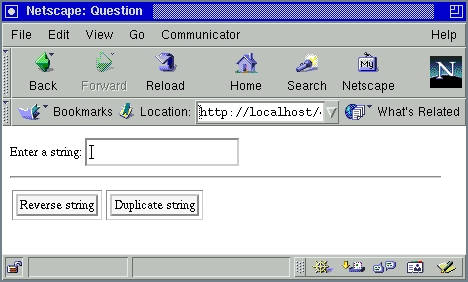
\includegraphics[scale=0.6]{PICTURES/revdup.jpg}
\end{center}\vspace{-3ex}
\caption{A simple string reverse/duplication form\label{fig-revdup}}
\end{figure}
%
\begin{curry}
rdFormContents :: [HtmlExp]
rdFormContents =
  [htxt "Enter a string: ", textfield tref "", hrule,
   button "Reverse string"   revhandler,
   button "Duplicate string" duphandler]
 where
   tref free

   revhandler env = return $ page "Answer"
     [h1 [htxt $ "Reversed input: " ++ reverse (env tref)]]

   duphandler env = return $ page "Answer"
     [h1 [htxt $ "Duplicated input: " ++ env tref ++ env tref]]
\end{curry}
%
Note the simplicity of retrieving values entered into the form:
since the event handlers are called with the appropriate environment
containing these values (parameter \ccode{env}),
they can easily access these values
by applying the environment to the appropriate HTML reference,
like \ccode{(env tref)}.

So far we have the definition of a form, but how can such forms
be embedded in an HTML page?
Note that a form has two different purposes:
%
\begin{enumerate}
\item
A form defines the layout and input fields shown to the user.
\item
A form defines the reaction via handlers when it is submitted.
\end{enumerate}
%
For this purpose, the library \code{HTML.Base}
distinguishes between a \emph{form definition} and
its actual \emph{use}.
For this purpose, forms must be defined as top-level entities
(which will be compiled by \code{curry2cgi}).
For this purpose, there is a constructor \code{simpleFormDef}
(other constructors are shown later):
%
\begin{curry}
simpleFormDef :: [HtmlExp] -> HtmlFormDef ()
\end{curry}
%
This operation wraps a form layout, possibly containing
input elements and event handlers, into a form definition
(the type argument of \code{HtmlFormDef} will be discussed later).
For instance, we turn our form above into a form definition by
%
\begin{curry}
rdFormDef :: HtmlFormDef ()
rdFormDef = simpleFormDef rdFormContents
\end{curry}
%
A defined form can be embedded into an HTML page
by wrapping the form definition with operation
\begin{curry}
formElem :: HtmlFormDef a -> BaseHtml
\end{curry}
Hence, the following code defines an HTML page
containing our form:
\begin{curry}
rdPage :: IO HtmlPage
rdPage = return $ page "String reverse/duplicate" [formElem rdFormDef]
\end{curry} % $
%
By defining the form together with the various handlers
in one top-level entity, forms are more reliable compared
to a separate definition of HTML structures and scripts to process them.
The advantage of distinguishing a form definition from its actual use
is that we can use a form in any HTML document,
in particular, recursively in the answer computed by an event handler.
For instance, a form to compute the length of
an input string and showing the form again in the answer can be defined
as follows \proghref{stringlength}{Program}:
\begin{curry}
lengthForm = simpleFormDef
  [htxt "Enter a string: ", textField ref "", button "Length"
    (\env -> return $ page "Answer"
               [h1 [htxt $ "Length: " ++ show (length (env ref))],
                hrule, formElem lengthForm])]
 where ref free

main :: IO HtmlPage
main = return $ headerPage "String length" [formElem lengthForm]
\end{curry} % $


\section{Stateful Forms}

The simple HTML forms presented so far are quite limited.
Form definitions are top-level entities so that their
layout is fixed, i.e., they cannot show data
from a possible usage context,
e.g., database entities or authentication data.
In order to make forms more flexible, it should be possible
that forms access some state to be shown in the form.
Such \emph{stateful forms} need only to read data,
since the manipulation of data, e.g., updating a data base
depending on the user input,
is usually performed by the event handlers
(therefore, event handlers are of type \code{IO}).

To support stateful forms, the library \code{HTML.Base}
defines a monad \code{FormReader} with
operations to read data (see below), i.e.,
the \code{FormReader} monad is a restriction of the \code{IO} monad
where only read operations are supported.\footnote{The restriction
to read operations is necessary since forms might be executed
several times, e.g., to construct the form layout,
to start an event handler, or if the form
has multiple occurrences in a web page.
Thus, a form should not change the environment.
Changes are only performed by the activation of some event handler.}
Thus, a stateful form consists of a \code{FormReader} action
to read data of some type \code{a} and an operation which maps
values of this type into an HTML form.
The library \code{HTML.Base} supports the definition
of stateful forms by the form constructor operation
%
\begin{curry}
formDef :: FormReader a -> (a -> [HtmlExp]) -> HtmlFormDef a
\end{curry}
%
Therefore, an operation of type \code{HtmlFormDef$\;$a}
specifies a form which reads some data of type \code{a}
and use this data to generate the actual HTML form.

In order to define a stateful form, we need an operation
of type \code{FormReader$\;$a}.
A difficulty in web programming is the fact that HTTP
is a stateless protocol, i.e., each web page can be shown
several times and there are no connections between different web pages
to pass some state from one page to another.
This problem is solved in typical web applications
by a session concept where each user has its own session
where session-local data can be stored,
like the login name of a user or the contents of a virtual shopping basket.
A session concept can be implemented via cookies to identify
the client in a session.
To hide the details of session handling,
the package \code{html2} contains the library \code{HTML.Session}
which provides the following operations (the type variable \code{a}
denotes the type of session data):\label{sec:session}
%
\begin{curry}
getSessionData    :: (Read a, Show a) => SessionStore a -> a -> FormReader a
putSessionData    :: (Read a, Show a) => SessionStore a -> a -> IO ()
removeSessionData :: (Read a, Show a) => SessionStore a -> IO ()
\end{curry}
%
The type variable \code{a} specifies the type of session data.
The class constraints \code{Read} and \code{Show} are required
since the data is stored on the web server.
\ccode{SessionStore$\;$a} is the type of a top-level entity
referring to some memory cell containing session information of type \code{a}.
\code{getSessionData} retrieves information of the current session
(and returns the second argument if there is no information, e.g.,
in case of a new session),
\code{putSessionData} stores information in the current session,
and \code{removeSessionData} removes such information.
A session store containing data of type \code{a}
can be defined in a Curry program as a top-level entity
by using the constructor operation
%
\begin{curry}
sessionStore :: (Read a, Show a) => String -> SessionStore a
\end{curry}
%
The argument is a unique name (consisting of letters and digits)
for the session store in the web application.\footnote{Session stores
are implemented as persistent global entities, see Curry package \code{global},
which are stored in the file system of the server.}

In order to see an application of this concept,
we implement a simple number guessing game:
the client has to guess a number
known by the server (here: \code{42}), and for each number entered
by the client the server responds whether this number
is correct, smaller or larger than the number to be guessed.
If the guess is not right, the answer form contains an input
field where the client can enter the next guess.
Moreover, the number of guesses should also be counted
and shown at the end.
Hence, the session state contains the number of trials
and is defined as
%
\begin{curry}
trials :: SessionStore Int
trials = sessionStore "trials"
\end{curry}
%
The form definition consists of an action that reads the current
session data and the HTML form for this data \proghref{guess}{Program}:
%
\begin{curry}
guessForm :: HtmlFormDef Int
guessForm = formDef (getSessionData trials 1) guessFormHtml

guessFormHtml :: Int -> [HtmlExp]
guessFormHtml t =
  [htxt "Guess a number: ", textField nref "",
   button "Check" guessHandler]
 where
  nref free

  guessHandler env = do
    let n = read (env nref)
    if n==42
      then do
        removeSessionData trials
        return $ headerPage ("Correct! " ++ show t ++ " guesses!") []
      else do
        putSessionData trials (t+1)
        return $ headerPage ("Too " ++ if n<42 then "small!" else "large!")
               [formElem guessForm ]
\end{curry} % $
%
The form handler reads the user input from the HTML environment
(one could add an additional check whether the input is a number string)
and compares it with the ``secret'' number.
If it is equal, the session data is removed before returning the answer,
otherwise the session data is updated
so that the next form invocation gets the updated data.


\section{Example: A Web Questionnaire}

In many web applications, clients want to store
or update information on the server, e.g., by putting orders
for books, flight tickets, etc.
In this section we show an example where a client
can change persistent data stored on the web server.


\begin{figure}[t]
\begin{center}
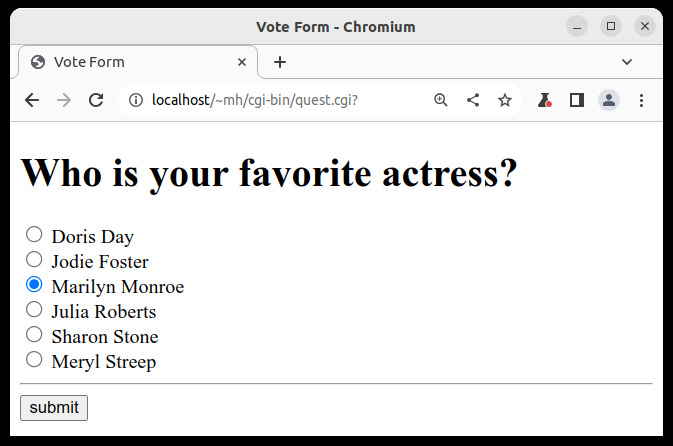
\includegraphics[scale=0.6]{PICTURES/quest.jpg}
\end{center}\vspace{-3ex}
\caption{A web questionnaire\label{fig-quest}}
\end{figure}

Consider the implementation of a web-based questionnaire
which allows the clients to vote on a particular topic.
Figure~\ref{fig-quest} shows an example of such a questionnaire.
The votes are stored on the web server.
The current votings are shown after a client
submits a vote (see Figure~\ref{fig-quest-answer}).

\begin{figure}[t]
\begin{center}
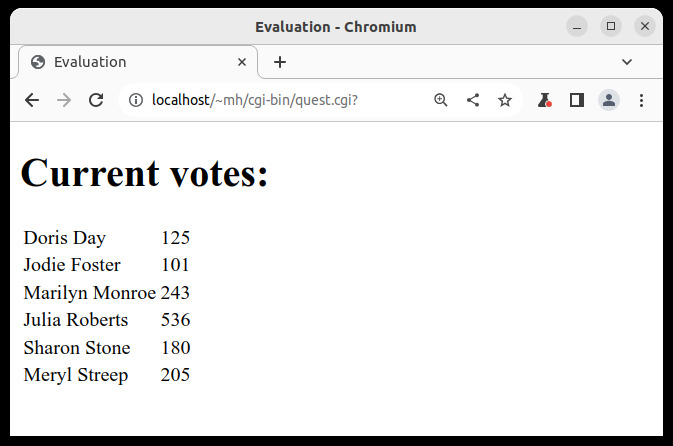
\includegraphics[scale=0.6]{PICTURES/quest_answer.jpg}
\end{center}\vspace{-3ex}
\caption{Answer to the web questionnaire\label{fig-quest-answer}}
\end{figure}

In order to provide an implementation that is easy to maintain,
we define the main question and the choices for the answers
as constants in our program so that they can be easily adapted
to other questionnaires:
\begin{curry}
question :: String
question = "Who is your favorite actress?"

choices :: [String]
choices = ["Doris Day", "Jodie Foster", "Marilyn Monroe",
           "Julia Roberts", "Sharon Stone", "Meryl Streep"]
\end{curry}
%
The current votes are stored in a file on the web server.
We define the name of this file as a constant in our program:
%
\begin{curry}
voteFile :: String
voteFile = "votes.data"
\end{curry}
%
For the sake of simplicity, this file is a simple text file.
If there are $n$ choices for voting, the file has $n$ lines
where each line contains the textual representation of the
number of votes for the corresponding choice.
Thus, the following operation reads
the vote file and returns the list of numbers in this file
or, if the file does not exist, initializes the vote file
and returns zeros
(the prelude function \code{lines}\pindex{lines} breaks
a string into a list of lines, where lines are separated by newline
characters, and the opposite function \code{unlines}\pindex{unlines}
concatenates a list of strings into lines).
%
\begin{curry}
readVoteFile :: IO [Int]
readVoteFile = do
  existnumfile <- doesFileExist voteFile
  if existnumfile
    then do vfcont <- readFile voteFile
            return (map read (lines vfcont))
    else do let nums = take (length choices) (repeat 0)
            writeFile voteFile (unlines (map show nums))
            return nums
\end{curry}
%
To update the vote file, we define \code{overwriteVoteFile}
that writes a list of numbers into the vote file.
The numbers are written into a new file that is moved to the vote file
in order to avoid an overlapping between reading and writing the same file.
\code{doesFileExist}\pindex{doesFileExist},
\code{removeFile}\pindex{removeFile}, and
\code{renameFile}\pindex{renameFile} are
I/O operations defined in the library \code{System.Directory}
(from package \code{directory})
to check the existence of a file, delete a file, and
rename a file, respectively.
%
\begin{curry}
overwriteVoteFile :: [Int] -> IO ()
overwriteVoteFile nums = do
  writeFile (voteFile ++ ".new") (unlines (map show nums))
  removeFile voteFile
  renameFile (voteFile ++ ".new") voteFile
\end{curry}
%
When a client submits a vote, we have to increment the corresponding
number in the vote file. This can be easily done by
reading the current votes and writing the votes
that are incremented by the auxiliary function \code{incNth}:
\begin{curry}
incNumberInFile :: Int -> IO ()
incNumberInFile voteindex = do
  nums <- readVoteFile
  overwriteVoteFile (incNth nums voteindex)
 where
  incNth []     _             = []
  incNth (x:xs) n | n==0      = (x+1) : xs
                  | otherwise = x : incNth xs (n-1)
\end{curry}
%
Now we have all auxiliary definitions that are necessary to define
the web script. First, we show the definition of
the HTML page \ccode{evalPage} that shows the current votes
(which produces the result shown in Figure~\ref{fig-quest-answer}).
The prelude function \ccode{zip}\pindex{zip} joins two lists
into one list of pairs of corresponding elements.
\begin{curry}
evalPage :: IO HtmlPage
evalPage = do
  votes <- exclusiveIO (voteFile ++ ".lock") readVoteFile
  return $ form "Evaluation"
   [h1 [htxt "Current votes:"],
    table (map (\(s,v) -> [[htxt s], [htxt $ show v]])
               (zip choices votes))]
\end{curry}
%
Note that we ensure the exclusive access to the vote file
by the use of the operation \code{exclusiveIO}.\footnote{The
operation \code{exclusiveIO} is defined in the library \code{System.IOExts}
contained in the package \code{io-extra}.}
This is necessary since there is not much control on the
access to web pages by clients.
In particular, the same CGI program might be executed
in parallel if two clients accessing them simultaneously.
This can cause problems if both read and update the same information.
Thus, it is mandatory to ensure exlusive data access
in web applications which might change data.
If the data is stored in files, it must be manually done, as above.
If the data is stored in databases, the database system ensures
the exclusive access but one has to take care
on the definition of transations.

Now we can define our form that allows the user to submit a
vote (see Figure~\ref{fig-quest}).
It uses radio buttons as input elements.
\label{radio button}\index{button!radio}
Radio buttons are lists of buttons where exactly one button
can be turned on. Thus, all buttons have the same HTML reference
but different values. When a form is submitted, the HTML environment
maps the HTML reference to the value of the selected radio button.
A complete radio button suite consists always of a main button
(\code{radioMain}) which is initially on and some further buttons
with the same HTML reference as the main button (\code{radioOthers})
that are initially off.
In our example, we associate to each button the index of the corresponding
choice as a value. The event handler \code{questHandler}
increments he appropriate vote number and returns the current votes
by the use of \code{evalPage}
\proghref{questionnaire}{Program}:
\begin{curry}
questForm :: HtmlFormDef ()
questForm = simpleFormDef $
  [h1 [htxt question],
   radioMain vref "0", htxt (head choices), breakline] ++
   concatMap (\(i,s) -> [radioOther vref (show i), htxt s, breakline])
             (zip [1..] (tail choices)) ++
   [hrule, button "submit" questHandler]
 where
   vref free

   questHandler env = do
     exclusiveIO (voteFile ++ ".lock")
                 (incNumberInFile (read (env vref)))
     evalPage

main :: IO HtmlPage
main = return $ page "Vote Form" [formElem questForm]
\end{curry}


\section{Finding Bugs}

Since debugging of CGI programs can be quite tedious,
here are some hints on how to debug CGI programs.

If the execution of the CGI program produces some run-time error
(e.g., access to a non-existing files), the error message
should be shown in the web page.
Furthermore, messages written to standard error output
are collected in the log file of the web script.
For instance, if the web script is stored at location
\code{cgi-bin/myscript.cgi},
the log file is \code{cgi-bin/myscript.cgi.log}.
Hence, if you want to put some debug output in your web script,
you should write it to standard error, e.g.,
%
\begin{curry}
hPutStrLn stderr "A log message"
\end{curry}
%
(where \code{hPutStrLn} and \code{stderr} are defined
in the standard library \code{IO}).

% If the execution of the CGI program does not produce a run-time error
% but simply fails (e.g., because of an incompletely defined function
% are a unification failure), you will probably see the message
% \ccode{No more solutions} in the web browser instead of the
% expected HTML document. For the purpose of debugging,
% it is often useful to see the subexpressions where a
% reduction was not possible but failed. In this case,
% you can  generate the CGI program by \ccode{makecurrycgi}\pindex{makecurrycgi}
% with the option \ccode{-debug}.
% This has the effect that some debugging code is inserted in the CGI
% program so that you can see the trace of all failed subexpressions
% in the browser (not formatted with HTML so that you should better
% view the source with your browser). Note that the debug option
% produces less efficient CGI programs so that it is better to
% use this option only when necessary.

The use of logic variables as references to input elements
in HTML forms ensures that typos in the name of references
can be detected by the compiler (e.g., resulting in an
``undeclared identifier'' error message), in contrast
to traditional approaches to CGI programming using plain strings
as references.
However, if we use the same logic variable for two different
input elements, this is not detected by the compiler
(which is not worse than traditional approaches where this
is also not detected) but results in a run-time error
that is not easy to understand due to the implementation
of the library \code{HTML.Base} in Curry.
In this case, the web script might fail with a message like
\ccode{No value found}.
Thus, you should check your source program for these possible errors
or add some debug output, as described above, to your script.


\section{Advanced Web Programming}
\label{sec-advanced-web-programming}

This section discusses some further features which are useful
for writing web applications in Curry.
\emph{URL parameters} can be exploited to write generic web scripts.
\emph{Cookies} are useful to store information about the client
between different web scripts.
\emph{Style sheets} can be used to modify and add new presentation styles
for web documents.


\subsection{URL Parameters}

In some situations it is preferable to have generic web scripts that
can be applied in various situations described by parameters.
For instance, if we want to write a web application that
allows the navigation through a hierarchical structure,
one does not want to write a different script for each different
level of the structure but it is preferable to write a single
script that can be applied to different points in the structure.
This is possible by attaching a parameter (a string)
to the URL of a script. For instance, a URL can have the form
\ccode{http://myhost/script.cgi?parameter} where
\ccode{http://myhost/script.cgi} is the URL of the web script
and \ccode{parameter} is an optional parameter that is passed
to the script.
A \emph{URL parameter}\index{URL!parameter}\index{parameter!URL}
can be retrieved inside a script
by the I/O action\pindex{getUrlParameter}
%
\begin{curry}
getUrlParameter :: IO String
\end{curry}
%
which returns the part of the URL following the character \ccode{?}.
Note that a URL parameter should be ``URL encoded'' to avoid
the appearance of characters with a special meaning.
The library \code{HTML.Base} provides the functions
\code{urlencoded2string} and \code{string2urlencoded}
to decode and encode such parameters, respectively.

As a simple example, we want to write a web script to navigate
through a directory structure. The current directory
is the URL parameter for this script. The script
extracts this parameter by the use of \code{getUrlParameter}
and shows all entries as a HTML list
\proghref{browsedir}{Program}
(the prelude function \code{mapM}\pindex{mapM} applies
a mapping from elements into actions to all elements of a list
and collect all results in a list):
%
\begin{curry}
showDirPage :: IO HtmlPage
showDirPage = do
  param <- getUrlParameter
  let dir = if null param then "." else urlencoded2string param
  entries <- getDirectoryContents dir
  hexps <- mapM (entry2html dir) entries
  return $ page "Browse Directory"
                [h1 [htxt $ "Directory: " ++ dir], ulist hexps]
\end{curry}
%
The I/O action \code{getDirectoryContents}\pindex{getDirectoryContents}
is defined in the library \code{System.Directory} (in package \code{directory})
and returns the list of all entries in a directory.
The function \code{entry2html} checks for an entry whether it
is a directory. If this is the case, it returns a link to
the same web script but with an extended parameter, otherwise
it simply returns the entry name as an HTML text
(\code{doesDirectoryExist}\pindex{doesDirectoryExist}
is defined in the library \code{System.Directory} and returns \code{True}
if the argument is the name of a directory):
%
\begin{curry}
entry2html :: String -> String -> IO [HtmlExp]
entry2html dir e = do
  direx <- doesDirectoryExist (dir ++ "/" ++ e)
  if direx
   then return [href ("?" ++ string2urlencoded (dir ++ "/" ++ e))
                     [htxt e]]
   else return [htxt e]
\end{curry}


\subsection{Cookies}

Cookies\index{cookie} are small pieces of information
(represented by strings) that are stored on the client's machine
when a client communicates to a web server via his browser.
The web server can sent cookies to the client together
with a requested web document. If the client wants to retrieve
the same or another document from the web server, the client's browser
sends the stored cookies together with the request for a document
to the browser.
Thus, cookies can be used to identify the client during a longer
interaction with the web server (also across various web scripts
stored on the same web browser).
Hence, cookies are used to implement session data
as described in Section~\ref{sec:session}.
In this section, we describe more details about cookies
if one is interested to implement his own session handling.

Basically, a cookie has a name and a value.
Both parameters are of type string.
Cookies can also have additional parameters to control their
lifetime, validity for different web servers or regions
on a web server etc (see definition of datatype
\code{CookieParam} in the library \code{HTML.Base}) which we will not describe
here. As the default, a cookie is a valid during the client's
browser session for all documents in the same directory or
a subdirectory in which the cookie was set.

The library \code{HTML.Base} provides two functions to set
and retrieve cookies.
As described above, a cookie is set by adding it with some
web page. For doing so, there is the function\pindex{addCookies}
%
\begin{curry}
addCookies :: [(String,String)] -> HtmlPage -> HtmlPage
\end{curry}
%
which adds a list of cookies, i.e., name/value pairs, to a web page.
These cookies are submitted with the page to the client's browser.
To retrieve cookies (that are previously sent),
there is an I/O action\pindex{getCookies}
%
\begin{curry}
getCookies :: IO [(String,String)]
\end{curry}
%
that returns the list of all cookies (i.e., name/value pairs)
sent from the browser for the current HTML page.

As a simple example, we want to use cookies to write a web application
where a user must identify himself and this identification is used
in another independent script. The identification is done
by setting a cookie of the form \code{("LOGINNAME",<name>)}
where \code{<name>} is the user's name.
We implement a ``login form'' that sets this cookie as follows
\proghref{logincookie}{Program}:
%
\begin{curry}
loginForm :: HtmlFormDef ()
loginForm = simpleFormDef
  [htxt "Enter your name: ", textField tref "",
   hrule,
   button "Login" handler
  ]
 where
   tref free

   handler env = return $
     addCookies [("LOGINNAME", env tref)] $
       page "Logged In"
            [h2 [htxt $ env tref ++ ": thank you for visiting us"]]

-- A web page containing the login form:
loginPage :: IO HtmlPage
loginPage = return $ page "Login" [formElem loginForm]
\end{curry}
%
First, the form asks the user for his name.
The cookie is set together with the acknowledgment page
(defined in function \ccode{handler}).

Now we can write another web script that uses this cookie.
This script shows the user's name or the string
\code{"Not yet logged in"} if the user has not used the
login form to set the cookie.
Using the function \code{getCookies}, the implementation
is quite simple (the function \code{lookup}\pindex{lookup}, defined in the
prelude, searches for a name in a name/value list;
it returns \ccode{Nothing} of the name was not found and
\ccode{Just v} if the first occurrence of the name in the list
has the associated value \code{v}; the prelude function
\code{maybe}\pindex{maybe} processes these two cases)
\proghref{logincookie}{Program}:
\begin{curry}
getNamePage :: IO HtmlPage
getNamePage = do
  cookies <- getCookies
  return $ page "Hello" $
    maybe [h1 [htxt "Not yet logged in"]]
          (\n -> [h1 [htxt $ "Hello, " ++ n]])
          (lookup "LOGINNAME" cookies)
\end{curry} %$
%
As mentioned above, cookies need special support on the client's
side, i.e., the web browser of the client must support cookies.
If cookies are essential for an application, one should check
whether the client allows the setting of cookies.
This can be done by trying to set a cookie and by checking
whether this was successful. For instance, one can modify
the above login script as folllows.
The first page immediately sets a cookie with name \ccode{SETCOOKIE}.
Then the handler checks whether this cookie has been sent by the
client's browser. If this cookie is not received, it returns a page
with the message ``Sorry, can't set cookies.'' instead of the
acknowledgment page which sets the cookie \ccode{LOGINNAME}
\proghref{checkcookie}{Program}:
\begin{curry}
loginPage :: IO HtmlPage
loginPage = return $
  addCookies [("SETCOOKIE","")] $ page "Login" [formElem loginForm]

loginForm :: HtmlFormDef ()
loginForm = simpleFormDef
  [htxt "Enter your name: ", textField tref "",
   hrule,
   button "Login" handler
  ]
 where
   tref free

   handler env = do
     cookies <- getCookies
     return $
       maybe (page "No cookies" [h2 [htxt "Sorry, can't set cookies."]])
             (\_ -> addCookies [("LOGINNAME",env tref)] $ page "Logged In"
                    [h2 [htxt $ env tref ++ ": thank you for visiting us"]])
             (lookup "SETCOOKIE" cookies)
\end{curry}


\subsection{Style Sheets}

The library \code{HTML.Base} provides various operations to add
style sheets to web pages (\code{pageCSS}) or to add
style classes to individual elements
(e.g., \code{style}, \code{textstyle}, \code{blockstyle}).
The package \code{html2} also contains libraries
to use \href{https://getbootstrap.com/}{Bootstrap} renderings
in web pages, see library
\href{https://cpm.curry-lang.org/DOC/html2-3.5.0/HTML.Styles.Bootstrap4.html}{HTML.Styles.Bootstrap4}
for more details.

%%% Local Variables: 
%%% mode: latex
%%% TeX-master: "main_pdf"
%%% End: 
% LocalWords:  HTML CGI URL stateful
